In the computation graph to be mapped, each node represents an instruction that needs to be placed onto a SE tile. 
The edges of the graph represent the data dependencies of the instructions. 
The nodes also contain information about the variables that need to be present in tile memories during instruction execution. 
All data needed for the instruction must be present at the tile for the instruction to be executed. 
The tiles can pass data to their neighbors and each tile can be configured with a different number of initiation intervals (II). 
Each II can be allocated to run a single instruction during program execution. 
After one cycle, the tiles will move on to the next II, with execution returning to first II after the last. 
All tiles run the instruction in the same II in parallel. 
Thus, whenever possible, independent instructions should be mapped to different tiles and same II to exploit parallelism. 
The first operation of each disconnected component of the computation graph (one component representing a synchronous flow) needs to be placed on different tiles. 
The SE device configuration and its constraints are modeled in a simulation environment and the reward function. 
Violating a constraint or placing instructions sub-optimally leads to a reduced reward whereas placements that optimally reduce total execution time of the graph are rewarded. 

Reinforcement learning tackles optimization problems by using the REINFORCE algorithm. 
It trains actor and critic models (represented as a neural networks). 
The actor model outputs actions (node placements) given an observation of the current state of the SE. 
The critic model is trained to predict the expected reward given an action in the current state. 
Proximal Policy Optimization (PPO) is a RL method widely used for continuous and discrete action problems. 
Our SE mapping task is formulated as a discrete action problem. 
In PPO, samples of SE state, actions performed, and rewards obtained at each time step are collected after executing the actions provided by the actor model in simulation. 
These samples are stored in a buffer that is used as data to train the models. In our case, the state is represented by a concatenation of an array of features of placed nodes, a selected node to be placed next and an embedding of the whole computation graph. An action is a tile location and an II count. The reward obtained is based on the number of cycles taken to execute all nodes. The actor model is trained to produce actions from sample states obtained during simulation and the critic model is trained to match the sampled rewards from the actions produced by the actor using a surrogate loss function. This sample and train process is repeated over various iterations. In this manner, the problem search space is explored using the reward function as a heuristic.  

In our neural network architecture, a graph neural network (GNN) is used to create embeddings from the computation graph, so that the RL models have information of the data dependencies of different nodes in the graph. 
An actor model with MLP layers and transformer encoder layers were evaluated in this work. Fig. 2 provides information about how the neural network is trained. 

\subsection{Streaming Engine environment}

% describe the Streaming engine environment
% state, obs, reward etc

\subsection{Model design}


\begin{figure}[h]
  \centering
  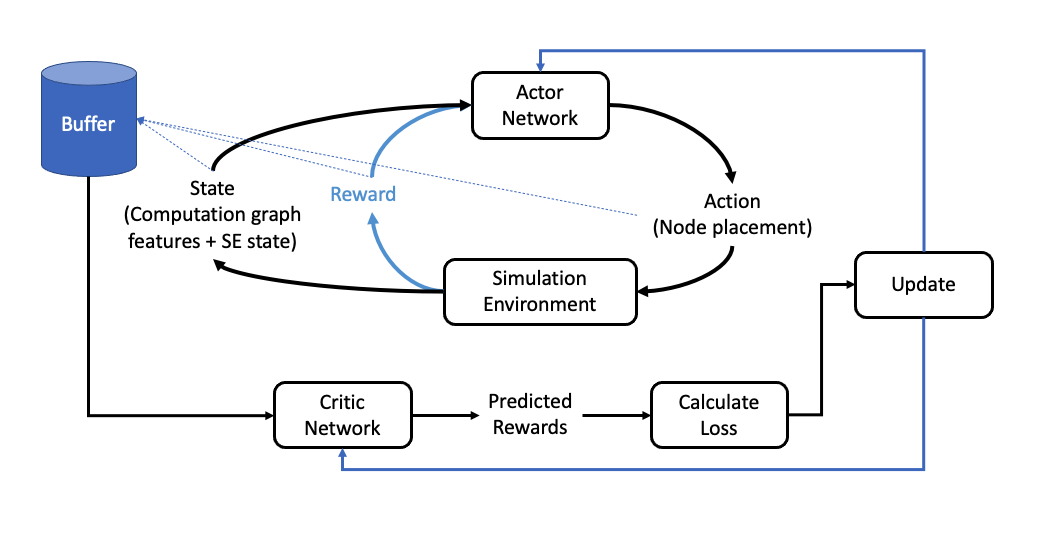
\includegraphics[width=\linewidth]{fig/ppo.png}
  \caption{Diagram of the RL model. }
\end{figure}


% pre post processing
% describe the graph neural network 
% attention module


\subsection{Reinforcement learning}

% describe the PPO training procedure

\cite{corr/SchulmanWDRK17}

\begin{figure}[h]
  \centering
  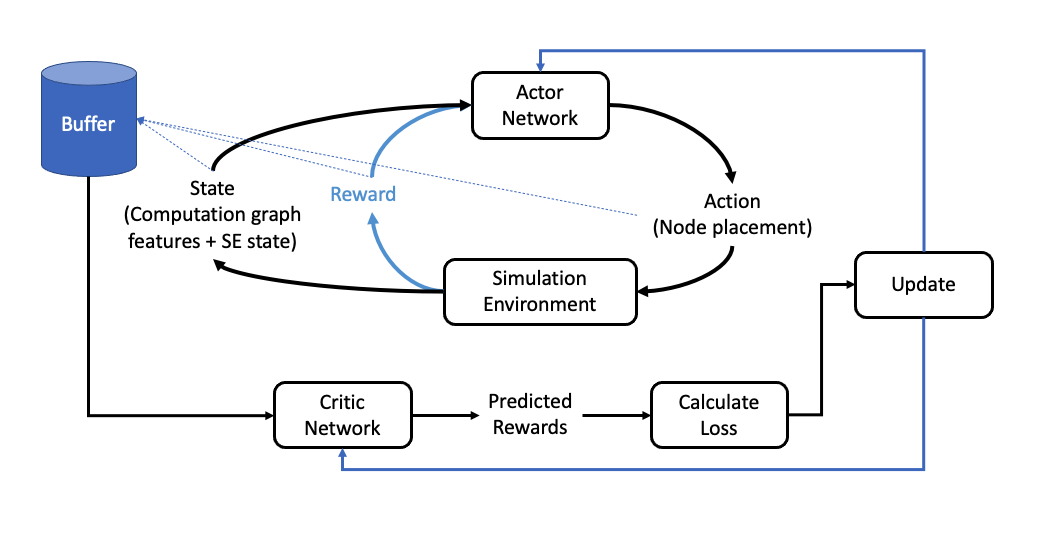
\includegraphics[width=\linewidth]{fig/ppo.png}
  \caption{Diagram of the RL framework showing the role of actor and critic networks during RL training. }
\end{figure}
